\documentclass{beamer}
\usetheme{focus}

\usepackage{todonotes}

\title{Design patterns}
\subtitle{Interpreter pattern}
\author{not-matthias}

\begin{document}
    \begin{frame}
        \maketitle
    \end{frame}

    % Section: What is the Interpreter Pattern?
    \section{What is the Interpreter Pattern?}

    \begin{frame}
        \begin{block}{Wikipedia says: }
            [...] the interpreter pattern is a design pattern that specifies how to evaluate sentences in a language. \cite{wikipedia_design_patterns}.
        \end{block}
    \end{frame}

    % Section: How does it work?
    \section{How does it work?}

    \begin{frame}{General}
        \begin{itemize}
            \item One class for each symbol
            \begin{itemize}
                \item Terminal
                \item Nonterminal
            \end{itemize}
        \end{itemize}
    \end{frame}

    \begin{frame}{Terminal Symbol}
        \todo[inline]{Write something}
        % https://en.wikipedia.org/wiki/Terminal_and_nonterminal_symbols
        % https://de.wikipedia.org/wiki/Terminalsymbol
    \end{frame}

    \begin{frame}{Nonterminal Symbol}
        \todo[inline]{Write something}
        % Replacable - nonterminal
        % https://en.wikipedia.org/wiki/Terminal_and_nonterminal_symbols
        % https://de.wikipedia.org/wiki/Nichtterminalsymbol
    \end{frame}

    % What problems can the Interpreter design pattern solve?
    \section{What problems can the pattern solve?}

    \begin{frame}
        \todo[inline]{Write something}
    \end{frame}


    % What solution does the Interpreter design pattern describe?
    \section{What solution does the pattern describe?}

    \begin{frame}{Abstract Syntax Tree}
        \begin{itemize}
            \item Define
        \end{itemize}
    \end{frame}

    \begin{frame}{Usage}
        \begin{itemize}
            \item Define a grammar for a simple language.
            \begin{itemize}
                \item By defining a \textit{Expression} class hierarchy with an \textit{interpret()} function.
            \end{itemize}
            \item Represent a sentence in the language with an AST made up of \textit{Expression} instances.
            \item Interpret a sentence by calling \textit{interpret()} on the AST.
        \end{itemize}
    \end{frame}

    % What solution does the Interpreter design pattern describe?
    \section{How can the pattern be used?}
    
    \begin{frame}{Applicability}
        \begin{itemize}
            \item Used when there's a language to interpret.
            \begin{itemize}
                \item Represent statements as AST
            \end{itemize}

            \item Works best when \textbf{the grammar is simple}.
            \begin{itemize}
                \item Use parsers for a large class hierarchy.
                \item Doesn't use an AST. Saves space and time.
            \end{itemize}

            \item Works best when \textbf{efficiency is not a critical concern}.
            \begin{itemize}
                \item More efficient when translating the parse tree to another form.
            \end{itemize}
        \end{itemize}

        % Source: https://github.com/iluwatar/java-design-patterns/tree/master/interpreter
    \end{frame}

    \begin{frame}{UML Class Diagram}
        \begin{figure}
            \centering
                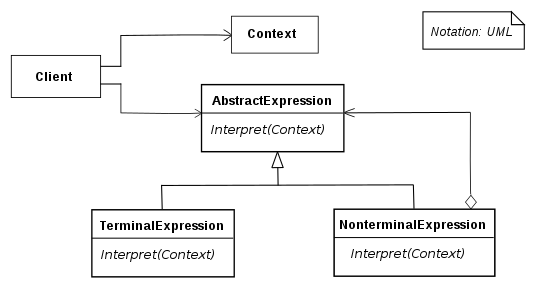
\includegraphics[width=0.8\textwidth]{figures/uml_class_diagram.png}
          \end{figure}
    \end{frame}
    
    \begin{frame}{Examples}
        \begin{itemize}
            \item \href{http://docs.oracle.com/javase/8/docs/api/java/util/regex/Pattern.html}{java.util.Pattern} 
            \item \href{http://docs.oracle.com/javase/8/docs/api/java/text/Normalizer.html}{java.text.Normalizer} 
            \item \href{http://docs.oracle.com/javaee/7/api/javax/el/ELResolver.html}{javax.el.ELResolver} 
            \item All subclasses of \href{http://docs.oracle.com/javase/8/docs/api/java/text/Format.html}{java.text.Format}
        \end{itemize}
    \end{frame}

    \begin{frame}{Other Examples}
        \begin{itemize}
            \item Specialized database query languages (e.g. SQL)
            \item 
        \end{itemize}
    \end{frame}

    % Demo
    \begin{frame}[focus]
        Demo.
    \end{frame}

    % End
    \begin{frame}[focus]
        System.out.prinln("Thanks.");
    \end{frame}

    % Appendix
    \appendix
    \begin{frame}{References}
        \nocite{*}
        \bibliography{references-bibliography}
        \bibliographystyle{plain}
    \end{frame}
    
\end{document}